\documentclass[11pt]{article}

\newcommand{\xautha}{Luca Mella}
\newcommand{\xauthb}{Daniele Bellavista}
\newcommand{\xtitle}{Emotime: Recognizing emotional states in faces}

\usepackage{amsmath}
\usepackage{placeins}
\usepackage{float}
\usepackage{ifpdf,ifluatex}
\ifluatex
\usepackage{fontspec}
\else
\usepackage[utf8x]{inputenc}
\fi

\usepackage{url}
\ifpdf
\usepackage{hyperref}
\hypersetup{unicode=true,
    pdftitle={\xtitle},
    pdfauthor={\xautha, \xauthb},
}
\fi

\usepackage{chngcntr}
\counterwithin{figure}{subsection}
\counterwithin{table}{subsection}

\usepackage{xspace}
\usepackage[usenames,dvipsnames]{xcolor}
\usepackage{graphicx}

\usepackage{listings}
\lstset{%
  breakatwhitespace=false,
  breaklines=true,
  captionpos=t,
  extendedchars=true,
  literate= {à}{{\`a}}1
            {η}{{$\eta$}}1
            {μ}{{$\mu$}}1
            {ρ}{{$\rho$}}1,
  frame=single,
  keepspaces=true,
  basicstyle=\ttfamily\footnotesize,
  keywordstyle=\color{blue},
  commentstyle=\color{OliveGreen},
  stringstyle=\color{RedOrange},
  numbers=left,
  numberstyle=\tiny\color{CadetBlue},
  rulecolor=\color{black},
  showspaces=false,
  showstringspaces=false,
  showtabs=false,
  tabsize=2,
  title=\lstname
}

\usepackage{algorithm}
\usepackage{algorithmic}

\newcommand{\action}[1]{\texttt{#1}\xspace}
\newcommand{\code}[1]{{\small{\texttt{#1}}}\xspace}
\newcommand{\codescript}[1]{{\scriptsize{\texttt{#1}}}\xspace}

% Cross-referencing
\newcommand{\labelsec}[1]{\label{sec:#1}}
\newcommand{\xs}[1]{\sectionname~\ref{sec:#1}}
\newcommand{\xsp}[1]{\sectionname~\ref{sec:#1} \onpagename~\pageref{sec:#1}}
\newcommand{\labelssec}[1]{\label{ssec:#1}}
\newcommand{\xss}[1]{\subsectionname~\ref{ssec:#1}}
\newcommand{\xssp}[1]{\subsectionname~\ref{ssec:#1} \onpagename~\pageref{ssec:#1}}
\newcommand{\labelsssec}[1]{\label{sssec:#1}}
\newcommand{\xsss}[1]{\subsectionname~\ref{sssec:#1}}
\newcommand{\xsssp}[1]{\subsectionname~\ref{sssec:#1} \onpagename~\pageref{sssec:#1}}
\newcommand{\labelfig}[1]{\label{fig:#1}}
\newcommand{\xf}[1]{\figurename~\ref{fig:#1}}
\newcommand{\xfp}[1]{\figurename~\ref{fig:#1} \onpagename~\pageref{fig:#1}}
\newcommand{\labeltab}[1]{\label{tab:#1}}
\newcommand{\xt}[1]{\tablename~\ref{tab:#1}}
\newcommand{\xtp}[1]{\tablename~\ref{tab:#1} \onpagename~\pageref{tab:#1}}

\begin{document}
\title{\xtitle}
\author{\xautha\\\xauthb}

\maketitle

\section{Approach and Technical Details}

% TODO: describe the elaboration pipeline
The general approach followed in this class project is based on the one adopted in \cite{Littlewort04dynamicsof,Bartlett06fullyautomatic}, where several concepts and algorithms are mixed and pipelined in order to achieve the not trivial task of the emotional states recognition. The methodology proposed on these papers is the following:

\begin{itemize}
\item Face detection and extraction
\item Facial features extraction via bank of Gabor filters.
\item Training several binary \emph{AdaBoost} classifiers with the labelled data (e.g.\ emotion labels).
\item Extraction of the most relevant features emerged after the training.
\item Most relevant facial features extraction based on valuable features observed.
\item Training several binary \emph{SVM} classifiers with the labelled data (e.g.\ emotion labels), using only most relevant features.
\end{itemize}

During project development we \emph{did not} rigidly follow the pipeline above for several pragmatical reasons, mainly related to the limited amount of time available for the class project. We adopted an approach based on a simplified version of this methodology. In detail our approach is based on the following steps:

\begin{itemize}
\item Face detection and extraction
\item Facial features extraction via bank of Gabor filters.
\item Training several binary \emph{Boost} classifiers with the labelled data (e.g.\ emotion labels).
\item Training several binary \emph{SVM} classifiers with the labelled data (e.g.\ emotion labels).
\end{itemize}

Further detail about reasons that have driven us to this approach can be found in~\ref{res:issues}.\\

In the following paragraphs we resume main characteristics of algorithms and datasets adopted in our class project.

% \cite{Littlewort04dynamicsof}
% \cite{Bartlett06fullyautomatic}
% \cite{learningOpenCV2008}

\subsection{Face Detection}

Face area represent the region of interest (ROI) in the context of this project, so we firstly focused on how to detect faces in an image. This kind of task has been widely discussed in literature and several algorithm implementation exists, in our case we choose to adopt a \code{Haar feature based cascade classifier}\cite{Viola01rapidobject}, which is also part of the OpenCV framework.\\
This detection methodology use an huge amount of simple Haar features to train an \emph{AdaBoost} cascade classifier. In detail the concept involved are:

\begin{description}
\item[Haar Features] this kind of features are calculated in a small windows of the image, in this window a binary mask is virtually applied and the value of the feature is the difference between the sum of the pixel values above the part of the mask with value 1 and the sum of the other part. An example of this kind of feature in fig.\ref{fig:haar}.
\item[Boosting] is a supervised machine learning approach that uses an ensemble of weighted \code{weak classifiers}. Further details in~\ref{appr:boosting}.
\item[Cascade Classification] this classification approach is based on several classification step, in each step a different feature is considered and if a feature value doesn't match the trained model the process is aborted and further stages are not evaluated.
\end{description}

\begin{figure}[!b]
\centering
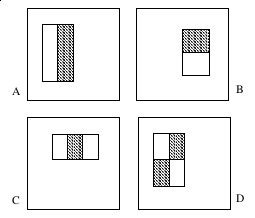
\includegraphics[width=4cm]{images/haarfeatures.png}
\label{fig:haar}
\caption{Haar feature example from \cite{Viola01rapidobject} }
\end{figure}

The OpenCV implementation also support \emph{multiscale detection}, which performs several detection steps rescaling the input image in order to identify object with different size with respect to the training sample sizes. High performance is reached due to the use of the \emph{integral image} for feature calculation. With this approach a single haar-feature can be calculated with 3/4 lookups and a couple of arithmetic operations. The integral image is calculated with the following formula: $ ii(x,y) = \sum_{x' \leq x, y' \leq y}{ i(x',y') } $.\\

However, AdaBoost and Haar features are not the only choice, OpenCV implementation also support \emph{local binary patterns} based features and other boosting algorithms (eg. \code{RealBoost}, \code{GentleBoost}, \code{Discrete AdaBoost}, \ldots).

% \cite{Viola01rapidobject}

\subsubsection*{Face Rotation}

Our projects also implement a simple face rotation correction algorithm, which is based on the position of eyes detected via specifically trained cascade classifiers. Once eyes position is obtained a simple trigonometry calculation is performed in order to get the value of the angle between the eye-line and the x-axis, this value is then used for the definition of rotation matrix which is applied to the whole image.

\subsection{Gabor Filters}

Roughly speaking Gabor filters are \emph{linear} filter obtained by modulating a sinusoid with a \emph{Gaussian}, this kind of filters is typically used in image processing for tasks like edge detection, texture classification and face recognition\cite{gaborApplication}. These filters result particularly effective in case of a time-frequency analysis, which is an analysis technique that aims to study a signal in both time and frequency domain \emph{simultaneously}, due to multi-resolution\footnote{Multi-resolution is a method for orthonormal base creation by slicing the signal space into subspaces at different scales} and multi-orientation properties. One reason of the great success of this kind of filters is the discovery that simple cells in the human visual cortex can be modelled with this particular filter.

\begin{equation}
g(x,y;\lambda,\theta,\psi,\sigma,\gamma) = \exp\left(-\frac{x'^2+\gamma^2y'^2}{2\sigma^2}\right)\exp\left(i\left(2\pi\frac{x'}{\lambda}+\psi\right)\right)
\end{equation}

Where $x' = x \cos\theta + y \sin\theta$, $y' = -x \sin\theta + y \cos\theta$, $\lambda$ is the wavelength of the sinusoid, $\theta$ is the spatial orientation of the filter, $\phi$ is the phase offset, $\sigma$ is the standard deviation of the Gaussian support and $\gamma$ is the aspect ratio factor (eg. 1.0 for circular).

\subsubsection*{Gabor Energy Filters}
One of the basic way to deal with complex Gabor filter is to consider the magnitude of the filter response and considering the energy response of the filter. In our implementation we used the euclidean norm $\left \| g \right \|_2 = \sqrt{ g_{real}^2+g_{imag}^2 }$ due to the separate calculation of both imaginary and real part.

\begin{figure}[!h]
\centering
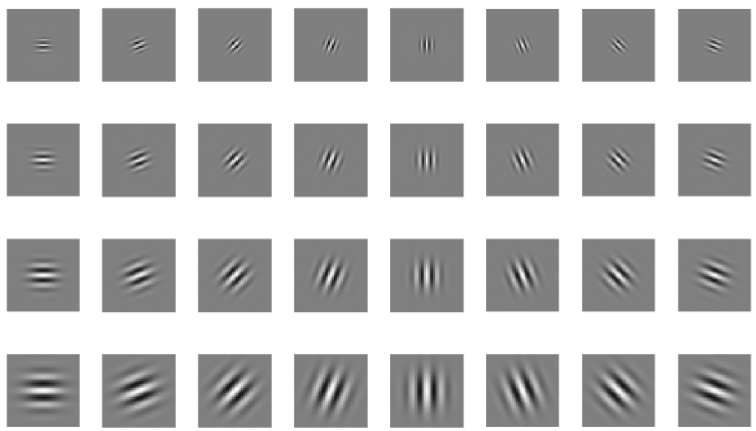
\includegraphics[width=12cm]{images/gabor.png}
\label{fig:gabor}
\caption{Magnitude of a Gabor filter bank from \cite{gaborApplication} }
\end{figure}

% \cite{gaborTutorial}
% \cite{gaborApplication}
% \cite{Lades93distortioninvariant}
\newpage
\subsection{Boosting}
\label{appr:boosting}

Boosting is a powerful learning concept that combines the performance of many ``weak'' classifiers to produce a ``strong'' one. For ``weak classifier'' is intended a generic classifier that performs slightly better than random choice, this non-restrictive requirement open new prospective for simple and computationally cheap classifiers (eg. simple thresholds). Boosting is some kind of meta-algorithm which can be applied in a lot of cases, using different classifiers, different weighting scheme or error functions. The general concept behind this supervised learning strategy is the weighting and re-weighting of the features in order focus on weak learner misprediction, and then weight their votes\cite{rojas2009adaboost}.\\

A classical case of boosting algorithm is the Adaptative Boost (\code{AdaBoost})\cite{Friedman98additivelogistic}, which one of the first boosting approaches proposed. For this reason we briefly introduce its behaviour and we introduce some variants.

\begin{algorithm}
\caption{Discrete AdaBoost algorithm (binary classification)} 
\label{alg:adaboost}
\begin{algorithmic}
\STATE $i=1 \ldots T$ training data, $x_i$ is sample and $y_i \in \{-1,+1\}$ is label
\STATE $w_{i}^{(1)}=1$ is the initial weight of $x_i$
\STATE $N$ iteration number
\STATE $M$ classifier number
\STATE $W$ is the sum of weights of all data points
\STATE $W_e$ is sum of weight of data where considered classifier yields wrong label
\FOR{$i \in 1 \ldots N$ } 
%	\FOR{$m \in 1,\ldots,M$ } 
		\STATE find classifier $k_{m}(x)$ which minimize $W_e=\sum_{y_i \neq k_m(x_i)}{w_{i}^{(m)}}$
		\STATE set weight of classifier to $\alpha_{m}=\frac{1}{2}ln(\frac{1-e_m}{e_m}) $, where $e_m=W_e/W$
		\IF{$k_m(x_i) $ is a miss} 
	 		\STATE update weights $w_{i}^{(m+1)}=w_{i}^{(m)}e^{\alpha_m}=w_{i}^{(m)}\sqrt{\frac{1-e_m}{e_m}}$
		\ELSE
			\STATE update weights $w_{i}^{(m+1)}=w_{i}^{(m)}e^{-\alpha_m}=w_{i}^{(m)}\sqrt{\frac{e_m}{1-e_m}}$
 		\ENDIF
%\ENDFOR
\STATE output $sign( \sum_{m \in 1 \ldots M}{ \alpha_m k_m (x)} )$
\ENDFOR
\end{algorithmic}
\end{algorithm}

OpenCV framework implements several AdaBoost variants like \code{Real AdaBoost}, where weak classifiers may express class probabilities $p_m(x)$ instead of $\{-1,+1\}$ values, and \code{Gentle AdaBoost} which updates weight differently $\alpha_{m}=P(y_i=1|x_i)-P(y_i=0|x_i)$. 

% \cite{rojas2009adaboost}
% \cite{Friedman98additivelogistic}

\subsection{SVM}

Support Vector Machine (\emph{SVM}) is a machine learning approach that
 constructs an hyperplane, which maximizes the distance between the training
 data of any class, performing a classification.
 
 Since results in \cite{Littlewort04dynamicsof} show that linear SVM performs
 slightly better than non-linear approaches, we used only \emph{Linear SVM} for
 its faster training speed. Specifically, we used the linear SVM implementation
 of \emph{OpenCV}, which realizes a \emph{C-Support Linear SVM}, or \emph{Linear
 SVM} with \emph{Soft Margin}.
 
 \begin{align}
   \min & \frac{1}{2} \boldsymbol{\omega}^T \boldsymbol{\omega} + C*\sum_{i=1}^l \xi_i\\
   & y_i * (\boldsymbol{\omega}^T \phi(\textbf{x}_i) + b) \geq 1 - \xi_i,\\
   & \xi_i \geq 0, i = 1, \dots, l
   \label{mt:lin_svm}
 \end{align}
 
 Where $\boldsymbol{\omega} \cdot \textbf{x} - b = 0$ is the hyperplane:
 $\boldsymbol{\omega}$ is the normal vector to the hyperplane and $\textbf{x}_i
 \in \mathbb{R}^n, i = 1,\dots,l$ are the training vector.  $y \in \mathbb{R}^l,
 y_i \in \{1, -1\}$ is a class indicator, $\xi_i$ is a non-negative slack
 variable measuring the degree of misclassification on $\textbf{x}_i$. The
 parameter $C$ gives a weight to these misclassification variables.

\subsection{Dataset}

Access to properly labelled data is not a trivial aspect when dealing with supervised machine learning algorithm, especially when you are not trained to label that kind of data. Emotion labelling is not a task that someone can improvise, training manual like \emph{Facial Action Coding System (FACS) Manual} exists and certification is required for preparing a scientifically valid dataset. For this reason we required access to the ``Cohn-Kanade Expression Database''\cite{Kanade2000} which contains 486 sequences from 97 posers, each sequence is tagged with FACS, contains facial feature tracking data and also have \emph{emotion labels}. \\

This dataset is considered is a ``must have'' from the academical community, in fact the lot of papers about topic related to \emph{faces} use at least this dataset. For this reason we choose it for our experimentation. 

% \cite{Kanade2000}

\newpage


\section{Parameters}

In this section we will discuss the parameter used for the algorithm adopted in the class project

\subsection{Face Detection Parameters}

OpenCV support several parameter for multi-scale detection, from the classifier to use, to scale factor and minimum object size. We performed several test using a quick and dirty python script to test which values provide good accuracy. After some empirical test we figured out that considering a 640x480 figure as the minimum face size of size of 120x200 produces good detection (face/image ratio is nearly 10\%). But for ensuring to detect all possible treatable faces for our system we setted up a minimum size of 30x60, this value is related to the resizing performed before feature extraction, in our experiments we chose 48x48, as performed also in\cite{Littlewort04dynamicsof}. So at the moment we decided to ignore the computational overhead introduced by this choice. \\

In the eyes detection step we decided to set the minimum object threshold to a dynamical value calculated using knowledge of face area size and a qualitative estimation of the human face proportions, in detail we consider that the width of an eye cannot be smaller than $\frac{1}{5}$ of the face width.\\

Also we tried several face detector in order to see which one fits better our purposes, for example we considered the \emph{haarcascade\_ frontalface\_default.xml} and the \emph{haarcascade\_frontalface\_cbcl1.xml}. The latter is interesting because it detects the inner part of the face, discarding the surrounding. This choice has side effects on results\ref{res:issues}.

\subsection{Gabor Kernels Parameters}

Gabor parameters selection is one of the most delicate part of the tuning process, it directly affects the features evaluated for the emotional state classification. Hopefully \cite{Littlewort04dynamicsof, Bartlett06fullyautomatic, Lades93distortioninvariant} provide some hints on the Gabor bank parameters that can be used to achieve good results, in detail the number of $\lambda$ (wavelength) to use, number of $\theta$ (orientation) and some clues about interesting wavelength ranges are provided:

\begin{itemize}
\item $\lambda \in ( \frac{\pi}{32} \ldots \frac{\pi}{2} ) $ as suggested in \cite{Lades93distortioninvariant}
\item $\theta \in ( 0 \ldots \frac{\pi}{2} )$
\item suggested 5 $\lambda$ and 8 $\theta$ subdivisions
\item same aspect ration $\gamma$ for each kernel in the bank
\end{itemize}

However despite these indications we decided to adopt a flexible approach by keeping subdivision number configurable in order to be able to refine parameters in further development stages. \\
Least, no clear indication about the size of the kernel, so we decided to support multiple kernel size ranging from $7$ to $17$, this values have been fixed in the first testing phase, using the developed Gabor utilities for visualizing the resulting bank. 

\subsection{Boosting Parameters}

Boosting parameters were considered in the early development stages and have ignored in the latest phases due to the huge amount of time needed for \code{AdaBoost} training. However parameters choice involves:

\begin{itemize}
\item algorithm variant to use, in our case \code{Real AdaBoost}, \code{Discrete AdaBoost} and \code{Gentle AdaBoost} 
\item classifier trim weight, as the lower accepted weight for a weak classifier
\item depth of the trained decision tree
\end{itemize}

We have no clues about this parameters so we tried several configuration and the better results have been obtained via \emph{Gentle AdaBoost}, trimming weak classifiers provide a speed-up but it is a sensible operation due to distribution of classifier weights. However, as reported in~\ref{res:issues} we have temporary dismissed the boosting approach due to lack of time.

\subsection{SVM Parameters}

Linear SVM with soft max has only one parameter, the value \emph{C}, which
defines how much to consider the misclassification. Since we hadn't any
validation set, we couldn't verify how much this value could affect the train.
We decided to leave $C=0.5$, for no particular reason.

\subsection{Multiclass Strategies}

Each classification algorithm adopted works only for binary classification tasks, and our problem involves 7 distinct classes. For this reason we follow the indications in \cite{Littlewort04dynamicsof, Bartlett06fullyautomatic} and implement a quite general support building a voting scheme based multi-class classifier which rely on binary classifiers.\\
In detail we support multi-class training and detection in the following configurations:

\begin{itemize}
\item \emph{1 vs 1}, binary classifiers separate single classes each others
\item \emph{1 vs all}, separate a class from the others
\item \emph{many vs many}, separate groups of classes
\end{itemize}

Indication in papers suggest that \emph{many vs many} should be the better approach, so we use this parameter as the default one.


\section{Project Architecture}

The project is composed by the following entities:

\begin{description}
  \item[FaceDetector:] an utility class that extracts faces from images.
  \item[GaborBank:] generator of features using gabor filters.
  \item[Classifier:] generic 2-class classificator, which can be
    trained to predict a feature matrix.
  \item[EmoDetector:] using a set of classifiers, it realizes a multi-class
    detection for emotions.
  \item[GUI:] generic GUI that uses an EmoDetector to predict the emotion.
\end{description}

Instead of creating a single executable that does everything, we choose a
\emph{linux-like} approach of having a set of tools, where each of them
performs a single task.

Thus, we created a set of efficient tools, written in \code{C++}, which perform
training and detection, while high-level tasks such as data and training
organization are done by \code{Python} scripts.

\subsection{Face detection}

The face detection task is realized by the class \code{FaceDetector}. It uses
trained \emph{Haar Cascadesthe} classifiers to detect and crop the first face
from an image.

Since the face can be partially occulted or rotated around the principal axis,
mere detection is not enough. We implemented only the roll correction, by using
another \emph{Haar Cascadesthe} classifier to detect the eyes coordinates. If
the eye are not on the same axis, the image is rotated.

The face detection receives as input an image and outputs a matrix containing
the cropped and adjusted face.

\subsection{Gabor bank}

The class \code{GaborBank} is a generator and container of \code{GaborKernel}.
It permits the generation of various Gabor kernels with different orientations,
dimensions and wavelengths.

Once filled, \code{GaborBank} can filter images, returning a matrix that
contains a stack of images, one for each filter present in the bank.

\subsection{Classifier}

\code{Classifier} is a generic 2-class classificator, which can be trained to
predict a feature matrix. The specializations classes we implemented are
\code{SVMClassifier} and \code{AdaBoostClassifier}.

The training set is composed by \emph{negative} (class 0) and \emph{positive}
(class 1) samples. The output is a trained classifier. We used the
\emph{OpenCV} \code{CvSVM} and \code{CvBoost}, which permit to save and load
their internal state.

\subsection{Emotion detector}

Once the 2-class classifiers are trained, they can be used together to realize
a multi-class classifiers. This goal is achieved by \code{EmoDetector}. It is
composed by multiple \code{Classifier} and combines their prediction in various
ways to detect the emotion.

The input is an image, which is preprocessed: the face is extracted and then
features are computed. Then result is the detected emotion with its prediction
score.

\subsection{GUI}

The GUI is realized using the \emph{OpenCV} API. A generic GUI (\code{AGui}) is
composed by a \code{FacePreProcessor}, which extracts features from images, an
\code{EmoDetector} and a \code{ACapture}.

An \code{ACapture} is a generic frame capture. The specializations we
implemented permit the capture from videos, images and webcams.

\subsection{Tools and scripts}

Tools are \code{C++} programs performing high-performance tasks. In order
to be generic, they require every algorithm parameter as input argument.

\begin{description}
  \item[facecrop\_cli] reads an image and output a new image with the cropped
    face. It performs also eye-adjusting.
  \item[gaborbank\_cli] reads an image and output a file containing the
    extracted features.
  \item[train\_cli] reads a training file, trains a classifier and writes the
    trained state in an output file in \emph{xml} format.
  \item[emo\_detector\_cli] reads images and detect emotions using trained
    classifiers.
  \item[emotimegui\_cli] capture the webcam and performs real-time emotion
    detection.
\end{description}

The duty of python scripts is to organize the training process, by using the
\code{C++} tools. The configuration, such as tools name and algorithm
parameters, are read from a configuration file.

\begin{description}
  \item[datasetInit.py] initializes the directory hierarchy needed by the
    training process. This directory is called \code{dataset} directory.
  \item[datasetFillCK.py] fills the \code{dataset} with images from the CK database.
  \item[datasetCropFaces.py] applies the facecrop tool to the images, saving
    them in the \code{dataset}.
  \item[datasetFeatures.py] uses the gaborbank tool to extract features from
    the faces. The features are saved as \emph{yml} files.
  \item[datasetPrepTrain.py] prepares the training files by combining the
    features files using various strategies. The output are \emph{csv} files
    containing the positive and negative samples.
  \item[datasetTrain.py] iterates the \emph{csv} training files and launch a
    multi-threading training using the train tool. Their output is trained
    classifiers, which are saved in the \code{dataset} as \code{xml} files.
  \item[datasetVerifyPrediction.py] uses the emo\_detector tool to verify the
    prediction of the trained classifiers. We don't have a \emph{validation
    set}, so we just test the prediction on the \emph{training set}.
\end{description}


\section{Results}

We performed training with several dataset configurations, but here we'll report only the most significant, however the reader may find implementation details, source code, trained models and log at \url{https://github.com/luca-m/emotime/}.

\subsection{Training Results}

Generalization performance is not formerly available due to the lack of a meaningful validation set\ref{res:issues}, so any generalization performance consideration should be taken as qualitative indications. Having said that, we reported good performance in the detection of ``happiness'', ``anger'', ``disgust'', ``neutrality'' and ``surprise'', less effective is the detection of ``contempt'', ``sadness'' and ``fear''. We observed emotion detection happens on expression peeks which can be observed especially during face expression transitions, this behaviour could be caused by our current implementation of the binary classifiers: the SVM classifiers adopted provide a \emph{boolean information} about its prediction, an estimation of distance from the sample and the boundary hyperplane should enable a more gradual detection.

We also observed that the \code{1vsAll} multi-class method provide more less noisy detections during a live web-cam session, \code{1vsAllExt} mode instead is able to always predict a valid state for each frame processed, but sometimes it result to be more unstable during the expression transition.

\subsection{Issues}
\label{res:issues}

Here is a brief discussion about problems and issues in general which remain unsolved due to the limited amount of time available for this class project.

\subsubsection*{Training Samples Number}

One of the main problems noticed during testing on arbitrary video or webcam is that detection of some emotions is not as good as some other ones, a possible explanation relies on the limited amount of samples of the adopted dataset: some emotions have only 10/20 samples, which is certainly not a huge number.\\
Also the Cohn-Kanade Expression Database represents only the first step in several articles we have read, typically other dataset flanked to it (MMI, FERET, JAFFE, \ldots).

\subsubsection*{Validation Dataset}

The availability of a single, basic dataset did not give us the opportunity to calculate the confusion matrix on validation set for assessing generalization performance.
%Also gaining access to datasets is not properly immediate: not automated registration, licence agreement and university affiliation are necessary.

\subsubsection*{Boosting Training Time}

The training time of multiple AdaBoost classifiers with $O(10^4)$ features is not negligible, it took more than a day to complete the whole training process. For this reason, we chose to temporarily skip the feature selection approach based on the boosting results and focus on SVM with linear kernel.

This means that our performance is not optimal because we may calculate some features which are actually not crucial in the decision process, nevertheless real-time performance is achieved.

\subsubsection*{Face Detector Side Effect}

We empirically noted that the face detector adopted for training and detection has side effect on generalization performance, a more formal discussion is not possible due to the lack of validation dataset availability. However we noted that using \code{haarcascade\_frontalface\_default}, the face detection rate increases, but part of the ROI of the face is not useful for emotion detection due to the presence of part of background, hair and ears, giving worst generalization performance.

Using \code{haarcascade\_frontalface\_cbcl1}, only the inner part of the face is detected, this leads to a lower face detection rate but the ROI results more dense of meaningful features. Since we resize ROI to a 48$\times$48 rectangle, which are relatively small images, the effect of the trade-off described above is not negligible.

\subsection{Examples}

Following pictures represent screenshots captured during live test session with webcam and sample videos.

\begin{figure}
\centering
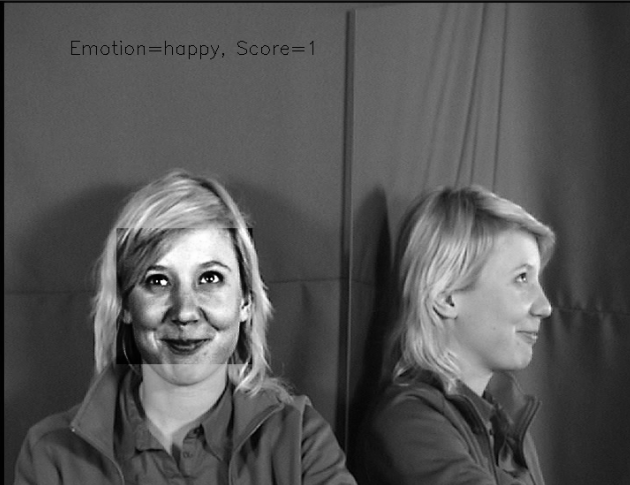
\includegraphics[width=7cm]{images/example_happy3.png}
\label{fig:example_happy3}
\caption{Happiness detection on a video from MMI dataset}
\end{figure}

\begin{figure}
\centering
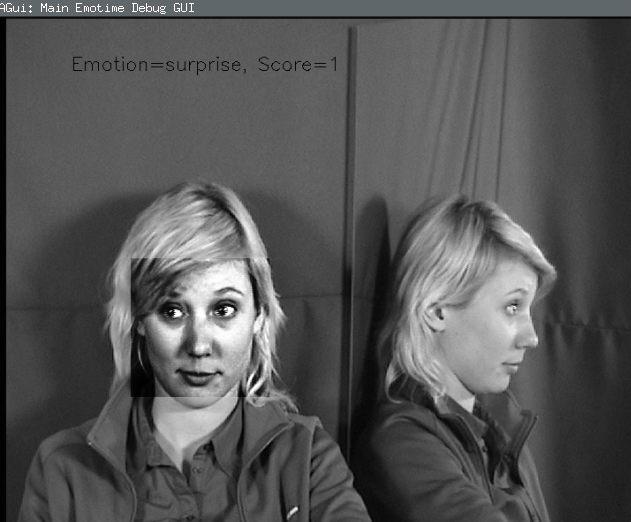
\includegraphics[width=7cm]{images/example_surprise.png}
\label{fig:example_surprise}
\caption{Surprise detection on a video from MMI dataset}
\end{figure}

\begin{figure}
\centering

\includegraphics[width=7cm]{images/example_happy1.png}
\label{fig:example_happy1}
\caption{Happiness detection on live webcam capture}
\end{figure}

\begin{figure}
\centering
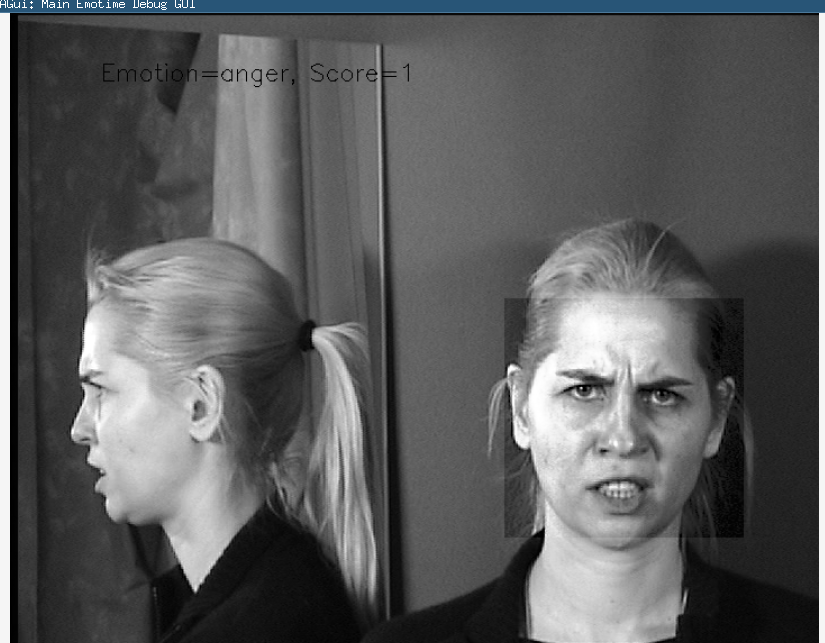
\includegraphics[width=7cm]{images/example_anger.png}
\label{fig:example_anger}
\caption{Anger detection on a video from MMI dataset}
\end{figure}

\begin{figure}
\centering

\includegraphics[width=7cm]{images/example_sad.png}
\label{fig:example_sad}
\caption{Sadness detection on live webcam capture}
\end{figure}

\begin{figure}
\centering
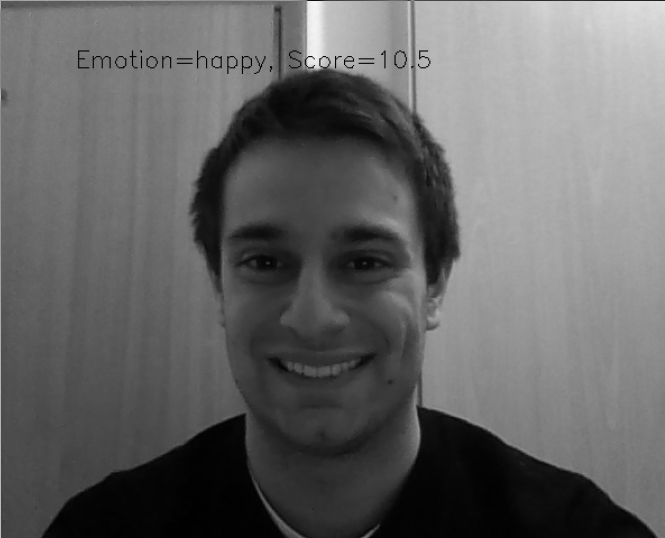
\includegraphics[width=7cm]{images/exampl_happy2.png}
\label{fig:exampl_happy2}
\caption{Happiness for happiness detection on live webcam capture}
\end{figure}

\begin{figure}
  \centering
  
\includegraphics[width=7cm]{./images/db_fear.png}
  \caption{Fear detection on live webcam capture}
  \label{fig:exampl_fear}
\end{figure}

\begin{figure}
  \centering
  
\includegraphics[width=7cm]{./images/db_anger.png}
  \caption{Anger detection on live webcam capture}
  \label{fig:exampl_anger}
\end{figure}

\begin{figure}
  \centering
  
\includegraphics[width=7cm]{./images/db_contempt.png}
  \caption{Contempt detection on live webcam capture}
  \label{fig:exampl_contempt}
\end{figure}

\begin{figure}
  \centering
  
\includegraphics[width=7cm]{./images/db_surprise.png}
  \caption{Surprise detection on live webcam capture}
  \label{fig:exampl_surprise}
\end{figure}
\newpage


\nocite{*}
\bibliographystyle{plain}
\bibliography{bib/bib}{}

\end{document}
